% ====================================================================
% GENERATED FILE — DO NOT EDIT.
%
% This file is auto-flattened by `make flatten` from the modular
% sources at paper/phantom_codes/{main.tex,sections/} (or the
% supplementary equivalent). Edit those instead; this file is
% overwritten on every `make snapshot-phantom_codes`.
%
% Source master: phantom_codes/main.tex
% Generator:     paper/scripts/flatten_paper.py
% ====================================================================

% Phantom Codes — main paper master file (IEEE J-BHI submission).
%
% Pure-LaTeX source. Section prose lives in sections/*.tex; xelatex +
% biber compiles directly with no pandoc step. To rebuild after
% editing any section:
%
%     cd paper && make phantom_codes
%
% Output: paper/phantom_codes/build/main.pdf (snapshotted to
%         paper/phantom_codes.pdf via `make snapshot-phantom_codes`).
%
% Editing model:
%   - All prose edits happen in sections/*.tex.
%   - This main.tex only changes when you add/remove/reorder sections,
%     change document class, add/remove packages, or restyle the title.
%
% Venue note: this preamble is configured for IEEE J-BHI (IEEEtran
% journal class, two-column, IEEE numerical citations). The JAMIA
% submission format is preserved in git history at commit d9ae5b2.

\documentclass[journal]{IEEEtran}

% ─── Fonts (XeLaTeX with fontspec) ─────────────────────────────────────
% IEEEtran defaults to Times-like fonts via pdflatex; under xelatex we
% use fontspec + STIX Two Text (Times-like OpenType with broad Unicode
% coverage). Mathematical glyphs (≥, ≤, →, ≈) are written in source as
% $\geq$, $\leq$, etc.
\usepackage{fontspec}
\setmainfont{STIX Two Text}

% ─── Tables, figures, lists ────────────────────────────────────────────
\usepackage{graphicx}
\usepackage{booktabs}
\usepackage{longtable}
\usepackage{array}
\usepackage{calc}
\usepackage{etoolbox}

% Long tables — apply footnote font size so wide tables (model ×
% prompting-mode × bucket layouts) fit within IEEE two-column width.
% IEEEtran is single-spaced by default; no setspace package needed.
\AtBeginEnvironment{longtable}{\footnotesize}

% ─── Math ──────────────────────────────────────────────────────────────
\usepackage{amsmath}
\usepackage{amssymb}

% ─── Bibliography ──────────────────────────────────────────────────────
% IEEE numerical citations [1], [2-4]. biblatex with biber backend;
% \autocite{Key} in section sources resolves at build time against
% references.bib.
\usepackage[backend=biber, style=ieee, sortlocale=en_US,
            maxnames=99]{biblatex}
\addbibresource{references.bib}

% ─── Links & references ────────────────────────────────────────────────
\usepackage[colorlinks=true,
            linkcolor=blue!60!black,
            citecolor=blue!60!black,
            urlcolor=blue!60!black]{hyperref}
\usepackage{xurl}

% ─── Code & quotes ─────────────────────────────────────────────────────
\usepackage{xcolor}
\usepackage{fancyvrb}
\usepackage{framed}
\usepackage{csquotes}

% ─── Pandoc legacy shim ────────────────────────────────────────────────
% \tightlist still appears in section sources.
\providecommand{\tightlist}{%
  \setlength{\itemsep}{0pt}\setlength{\parskip}{0pt}}

% ─── Title and author block (IEEE format) ──────────────────────────────
\title{Phantom Codes: Hallucination, Accuracy, and Cost in
LLM-Based Medical Concept Normalization}

\author{Brian~K.~Fung,~\IEEEmembership{PharmD,~MPH}%
\thanks{B.~K.~Fung is an independent researcher,
Brandon, FL, USA (e-mail: brian@briankfung.com;
ORCID: 0000-0002-5951-3770).}}

\markboth{IEEE Journal of Biomedical and Health Informatics,~Vol.~XX,
No.~X, 2026}%
{Fung: Phantom Codes: Hallucination, Accuracy, and Cost in LLM-Based
Medical Concept Normalization}

\begin{document}

\maketitle

% ─── Abstract (IEEE convention: plain paragraph, no structured headings)
\begin{abstract}
We evaluate the most recent frontier large language models (LLMs)
on medical concept normalization, separating fabrication of
non-existent codes from abstention as distinct failure modes, and
identify the (model, prompting-mode) configurations that combine
high accuracy with low per-prediction cost. We evaluate eight
frontier LLMs (Claude Opus 4.7, Sonnet 4.6, Haiku 4.5; GPT-5.5,
GPT-4o-mini; Gemini 2.5 Pro, 2.5 Flash, 3 Flash Preview) under
three prompting modes (zero-shot, constrained, retrieval-augmented)
against string-matching and frozen sentence-transformer baselines.
Inputs are Synthea-generated FHIR Conditions under four degradation
modes; a six-way outcome taxonomy separates fabrication from
abstention. On 125 unique Synthea Conditions across four
degradation modes, fabrication ranged from 0 to 5.6\% across
flagship configurations and from 0 to 12.8\% across sub-flagship
configurations. Constrained prompting eliminated fabrication for
every Anthropic and OpenAI model. Abstention proved more
consequential for some models: Gemini 2.5 Pro returned an empty
prediction on 88\% of zero-shot D4 inputs. Cost-per-correct varied
by a factor of 270 across the matrix; GPT-4o-mini in constrained
mode achieved the lowest cost at \$0.0003 per exact match.
Zero-shot LLM prompting is inferior to constrained and
retrieval-augmented grounding for medical concept normalization;
only the grounded configurations eliminated observed fabrication.
Cost-per-correct drives deployment selection: GPT-4o-mini
constrained leads at 94.2\% top-1 and \$0.0003 per correct, with
Claude Haiku 4.5 constrained as the higher-accuracy alternative
(96.8\%, \$0.0044). Both dominate the largest frontier model tested
(Opus 4.7, \$0.0133 per correct).
\end{abstract}

\begin{IEEEkeywords}
Natural language processing, International Classification of
Diseases, artificial intelligence, medical informatics,
reproducibility of results, large language models, hallucination,
semantic interoperability.
\end{IEEEkeywords}

% ─── Body ──────────────────────────────────────────────────────────────
% Each section is a hand-edited .tex file under sections/. The
% IEEE template does NOT use a separate title page or structured
% abstract page; sections/00_title_page.tex and sections/01_abstract.tex
% are JAMIA-format and not included in the IEEE build.

\section{BACKGROUND AND SIGNIFICANCE}\label{background-and-significance}

Medical concept normalization is the entity-linking task of mapping
in-text mentions of biomedical concepts like diagnoses, medications,
labs, and procedures to entries in a standardized ontology or
controlled vocabulary such as ICD-10-CM, LOINC, or RxNorm
\autocite{Miftahutdinov2021,Xu2022}. It sits at the foundation of
healthcare data interoperability. Errors propagate downstream: a
misassigned diagnosis code can shift a hospital's case-mix index,
mis-stratify a research cohort, or corrupt the training data of the
next generation of models. For most of the last decade, the state
of the art for automated coding came from supervised neural
classifiers trained on labeled clinical text
\autocite{Mullenbach2018,Huang2022}. The arrival of general-purpose
large language models has changed the deployment picture: foundation
models can in principle perform code prediction with no task-specific
fine-tuning. Two open questions motivated this work. Do the
fabrication findings reported on earlier model generations still
hold for the frontier models shipping today? And what does the cost
side of the deployment tradeoff look like for the configurations
that do work?

Concept normalization is also a load-bearing component of
\textbf{semantic interoperability}: the property that lets disparate
healthcare information systems exchange data in ways that preserve
clinical meaning, not just syntactic structure. Modern interoperability
stacks (HL7 FHIR, IHE profiles, the OMOP Common Data Model) presume
that values in coded fields resolve to entries in controlled
vocabularies (ICD-10-CM, LOINC, RxNorm, SNOMED CT); they break
silently when those resolutions fail. As clinical data warehouses
scale to support secondary use, multi-site cohort construction, and
FAIR data practices, automated terminology grounding becomes a
critical step in the harmonization pipeline. LLMs are a candidate
mechanism for that step. What determines whether they are viable in
production is not raw accuracy in isolation but the conjunction of
three properties: how often they fabricate codes that do not exist
(silently corrupting downstream harmonization), how often they
abstain (creating tractable gaps a reviewer can fill), and at what
per-prediction cost the resulting pipeline operates at scale.

The literature has documented the fabrication problem but on
generations that are now dated. Soroush et al.\ (2024) reported
that GPT-4 achieved only 46\% exact match on ICD-9 and 34\% on
ICD-10, with a substantial fraction of errors being non-existent
codes rather than real-but-wrong assignments
\autocite{Soroush2024}. Lee and Lindsey documented that LLMs
systematically struggle to distinguish real codes from
plausibly-formatted fakes \autocite{Lee2024}. Both findings are an
instance of the broader medical-hallucination phenomenon
\autocite{Kim2025,Ji2023}, and both predate Anthropic's Opus 4.7,
OpenAI's GPT-5.5, and Google's Gemini 3 Flash Preview. Whether the
fabrication rates reported on GPT-4 generalize to the current
generation has not been re-measured.

Cost is largely absent from the published evaluations. The field's
response to hallucination has been architectural: retrieval-grounded
pipelines \autocite{DasBaksi2024,Sarvari2025}, agentic walkers
\autocite{Motzfeldt2025}, neuro-symbolic verifiers
\autocite{HybridCode2025}, and broader benchmark expansions
\autocite{Almeida2025,Singh2025,Li2025,Gershon2025}. Across this
body of work, hallucination is rarely treated as an explicit
outcome, and per-prediction cost is rarely reported at all. As
LLM-augmented coding moves toward production deployment, the
operationally relevant question is which (model, prompting mode)
combination achieves a useful accuracy at a tolerable cost. The
literature does not yet answer that question.

We present \textbf{Phantom Codes}, whose primary contribution is a
reproducible evaluation framework for LLM-based terminology
grounding, demonstrated on the most recent frontier-model
generation. The framework has four reusable components. \emph{First},
a \textbf{six-way outcome taxonomy} in which fabrication of
non-existent codes (hallucination) and abstention
(\texttt{no\_prediction}) are explicit, mutually exclusive buckets;
the taxonomy generalizes to any closed-vocabulary grounding task
including LOINC and RxNorm. \emph{Second}, a \textbf{within-model
ablation} across zero-shot, constrained, and retrieval-augmented
prompting modes that holds the model and input fixed and varies
only whether a candidate list is provided, isolating ``wandering
off the menu'' from genuine ignorance. \emph{Third}, an
\textbf{abbreviation-stress mode (D4)} that replaces canonical
display strings with clinical jargon (T2DM, HTN, CKD-3) to expose
where string-matching baselines collapse and where genuine semantic
mapping is required; D4 functions as a robustness probe for any
LLM-grounding pipeline. \emph{Fourth}, \textbf{per-prediction cost
as a first-class outcome} alongside accuracy; we report cost-per-
correct (USD per exact-match outcome) as the deployment-relevant
normalization, computed from per-call token usage against published
per-token rates.

The empirical application of this framework spans 24 (model,
prompting-mode) configurations across Claude Opus 4.7, Sonnet 4.6,
and Haiku 4.5; GPT-5.5 and GPT-4o-mini; and Gemini 2.5 Pro, 2.5
Flash, and 3 Flash Preview --- several released within weeks of the
evaluation date. The headline matrix runs against Synthea-generated
FHIR Bundles \autocite{Walonoski2018}, a freely-redistributable
synthetic patient dataset that gives full reproducibility from a
pinned Synthea version and seed.
\section{MATERIALS AND METHODS}\label{materials-and-methods}

\subsection{Data}\label{data}

The headline evaluation matrix runs entirely against
Synthea-generated FHIR Bundles \autocite{Walonoski2018}, a freely-
redistributable synthetic patient dataset. 

\subsection{Cohort and label space}\label{cohort-and-label-space}

We restrict the cohort to ICD-10-CM codes in the CMS ACCESS Model
FHIR Implementation Guide v0.9.6 \autocite{CMS2026}. The Implementation
Guide defines two disease groups: \textbf{CKM} (cardiometabolic, covering
diabetes, atherosclerotic cardiovascular disease, and CKD stage 3)
and \textbf{eCKM} (extended cardiometabolic, covering hypertension,
dyslipidemia, prediabetes, and obesity). The headline matrix is
evaluated on a single Synthea-generated cohort of \textbf{125 unique FHIR
Conditions}, each materialized into four degradation modes for a
total of 500 EvalRecord items. Cohort generation is fully
deterministic: Synthea v4.0.0 \autocite{Walonoski2018} is run at a pinned
commit SHA with \texttt{seed=42}, producing patient bundles whose
Conditions are extracted, deduplicated per (patient, ICD code), and
filtered to ACCESS-scope codes via bundled value-set definitions.
Twelve unique ICD-10-CM codes appear in the cohort: obesity (\textasciitilde24\%),
prediabetes (\textasciitilde20\%), type 2 diabetes variants (\textasciitilde31\%), essential
hypertension (\textasciitilde14\%), and lipid disorders (\textasciitilde10\%).

\subsection{Models evaluated}\label{models-evaluated}

The headline matrix comprises 28 model configurations. These are:
three string-matching baselines (exact, fuzzy, TF-IDF), one frozen
sentence-transformer retrieval baseline, and 24 frontier LLM
configurations across three providers and three prompting modes.
Each LLM appears in \texttt{zeroshot}, \texttt{constrained}, and \texttt{rag}
configurations.

\begin{itemize}
\tightlist
\item
  \textbf{Anthropic} (3 × 3): Claude Haiku 4.5, Sonnet 4.6, Opus 4.7
\item
  \textbf{OpenAI} (2 × 3): GPT-5.5 (\texttt{gpt-5.5-2026-04-23}) and GPT-4o-mini
  \autocite{OpenAIModels2026}
\item
  \textbf{Google} (3 × 3): Gemini 2.5 Pro, Gemini 2.5 Flash, and Gemini 3
  Flash Preview (preview-status, disclosed as such) \autocite{GeminiModels2026}
\end{itemize}

Gemini 3.1 Pro Preview was excluded due to insufficient daily quota
at our API tier; a partial-coverage analysis appears in
Supplementary §S2. Per-token pricing for cost calculations was
sourced from each provider's documentation as of the evaluation date
\autocite{OpenAIPricing2026,GeminiPricing2026}.

\subsection{Prompting modes}\label{prompting-modes}

All LLMs are evaluated under three prompting modes that vary in how
much external structure is provided.

\begin{itemize}
\tightlist
\item
  \textbf{\texttt{zeroshot}}: a generic system prompt instructs the model to
  return the most likely ICD-10-CM code for the input, with no
  candidate list.
\item
  \textbf{\texttt{constrained}}: the system prompt additionally includes the
  full list of CMS ACCESS-scope candidate codes (with display
  strings) and instructs the model to choose only from that list.
  Mechanical schema enforcement (Anthropic forced tool use, OpenAI
  structured outputs, Google \texttt{response\_schema}) is applied across
  all modes; in \texttt{constrained} mode the menu itself is also passed
  in-prompt.
\item
  \textbf{\texttt{rag}}: a frozen sentence-transformer (\texttt{all-MiniLM-L6-v2})
  retrieves the top-k = 10 ACCESS-scope candidate codes most similar
  to the per-record input and injects only those into a
  constrained-style prompt.
\end{itemize}

The verbatim system and user prompts and per-provider tool-use and
schema configurations are reproduced in Supplementary §S1.

\subsection{Outcome taxonomy}\label{outcome-taxonomy}

Each per-record top-1 prediction is classified into one of six
mutually exclusive, exhaustive outcome buckets, ordered from best
to worst by deployment relevance:

\begin{enumerate}
\def\labelenumi{\arabic{enumi}.}
\tightlist
\item
  \textbf{\texttt{exact\_match}}: predicted code equals ground truth.
\item
  \textbf{\texttt{category\_match}}: predicted code is in the same ICD-10-CM
  3-character category as ground truth (e.g., E11.0 vs.~E11.9, both
  Type 2 diabetes).
\item
  \textbf{\texttt{chapter\_match}}: same ICD-10-CM chapter, different category.
\item
  \textbf{\texttt{out\_of\_domain}}: real ICD-10-CM code with no hierarchical
  relation to ground truth.
\item
  \textbf{\texttt{no\_prediction}}: model returned no usable prediction (empty
  array, refusal, or transient API failure that exhausted the SDK
  retry budget). The model fabricated nothing; it abstained.
\item
  \textbf{\texttt{hallucination}}: predicted code does not exist in the FY2026
  CMS ICD-10-CM tabular list (mechanically validated against the
  bundled validator).
\end{enumerate}

The \texttt{no\_prediction} and \texttt{hallucination} buckets capture
qualitatively different failure modes and are reported separately.
From a downstream-error perspective, abstention is generally
preferable to fabrication, since an abstaining model emits no
spurious code that downstream systems silently mishandle. Earlier work \autocite{Soroush2024}
collapses these into a single error bucket; the six-way split
surfaces the distinction that conflation hides.

\subsection{Cost tracking}\label{cost-tracking}

For every model invocation in our matrix the per-prediction CSV
records token usage, latency, and \texttt{cost\_usd} computed at runtime
against the versioned pricing snapshot in \texttt{configs/pricing.yaml}
\autocite{OpenAIPricing2026,GeminiPricing2026}. These infrastructure
metrics are recorded even when the prediction is wrong and serve
as the basis for the cost-per-correct normalization reported in
Results. Cost-per-correct (USD per exact-match outcome) combines per-call
price and per-call accuracy into a single number; we report it
alongside per-call cost because the two diverge when accuracy
drops.

\subsection{Statistical analysis}\label{statistical-analysis}

Per-(model, mode) outcome rates are reported as point estimates
with 95\% Wilson confidence intervals, which we prefer over
normal-approximation intervals because both small N and rates near
zero or one are common in our matrix (per-cell N = 125, and
constrained-mode hallucination rates approach 0\%). Within-model
paired comparisons across zero-shot, constrained, and RAG modes on
identical inputs are reported as exact McNemar tests on discordant
prediction pairs. Across-model and across-mode comparisons are
reported descriptively with overlapping or non-overlapping CIs. We
deliberately do not perform null-hypothesis significance tests
across the full grid, because the intended interpretation is
comparative deployment relevance rather than detection of any
single effect.
\section{RESULTS}\label{results}

\subsection{Cohort}\label{cohort}

The Synthea evaluation cohort comprises 125 unique synthetic FHIR
Conditions \autocite{Walonoski2018}, materialized into all four degradation
modes for a total of 500 records. Twelve unique ICD-10-CM codes
appear: obesity (E66.9; 24\%), prediabetes (R73.03; 20\%), type 2
diabetes variants (E11.x; 31\% combined), essential hypertension
(I10; 14\%), and lipid disorders (E78.x; 10\%). The matrix evaluates
28 model configurations.

\subsection{Outcome distribution}\label{outcome-distribution}

Two patterns dominate (per-cell N = 125; full table in
Supplementary §S2.1). Anthropic constrained and RAG modes achieve
zero fabrication across all sizes and all four degradation modes,
and GPT-4o-mini and GPT-5.5 in constrained or RAG mode match.
Fabrication concentrates instead in zero-shot prompting and varies
by model tier. Flagship models (Opus 4.7, GPT-5.5, Gemini 2.5 Pro)
range from 0\% to 5.6\% across all cells, with the maximum from Opus
zero-shot D3. Sub-flagship models (Sonnet 4.6, Haiku 4.5,
GPT-4o-mini, Gemini Flash variants) range from 0\% to 12.8\%, with
the maximum from GPT-4o-mini zero-shot D2. A pooled median
understates the spread, because D1 and D2 inputs expose the source
code and constrained or RAG cells are 0\% by design. Gemini 2.5
Pro's 0\% fabrication rate comes from abstention (95.2\%
no\_prediction at D4 zero-shot), not from correct answering.

\subsection{Failure-mode breakdown: hallucination and abstention}\label{failure-mode-breakdown-hallucination-and-abstention}

The literature historically conflates two failure modes:
fabrication of non-existent codes (hallucination) and abstention
(no\_prediction). They surface different patterns (Figure 1).
Table 1 reports both rates per cell as hallucination \% /
no\_prediction \%. Per-cell N = 125; Wilson 95\% CIs are ±3pp at 0\%,
±5pp at 5\%, and ±8 to ±9pp at 50\% (full CIs in §S2.2 to §S2.3).

\begin{table*}[!t]
\centering
\caption{Failure-mode breakdown by model and degradation mode. Each cell reports hallucination \% / no\_prediction \%.}
\begin{tabular}{@{}
  >{\raggedright\arraybackslash}p{(\columnwidth - 8\tabcolsep) * \real{0.2000}}
  >{\raggedright\arraybackslash}p{(\columnwidth - 8\tabcolsep) * \real{0.2000}}
  >{\raggedright\arraybackslash}p{(\columnwidth - 8\tabcolsep) * \real{0.2000}}
  >{\raggedright\arraybackslash}p{(\columnwidth - 8\tabcolsep) * \real{0.2000}}
  >{\raggedright\arraybackslash}p{(\columnwidth - 8\tabcolsep) * \real{0.2000}}@{}}
\toprule
\begin{minipage}[b]{\linewidth}\raggedright
Model (mode)
\end{minipage} & \begin{minipage}[b]{\linewidth}\raggedright
D1\_full
\end{minipage} & \begin{minipage}[b]{\linewidth}\raggedright
D2\_no\_code
\end{minipage} & \begin{minipage}[b]{\linewidth}\raggedright
D3\_text\_only
\end{minipage} & \begin{minipage}[b]{\linewidth}\raggedright
D4\_abbreviated
\end{minipage} \\
\midrule
claude-haiku-4-5 (constrained) & 0.0 / 0.0 & 0.0 / 0.0 & 0.0 / 0.0 & 0.0 / 0.0 \\
claude-haiku-4-5 (zeroshot) & 0.0 / 0.0 & 3.2 / 0.0 & 4.8 / 0.0 & 3.2 / 0.0 \\
claude-sonnet-4-6 (constrained) & 0.0 / 0.0 & 0.0 / 0.0 & 0.0 / 0.0 & 0.0 / 0.0 \\
claude-sonnet-4-6 (zeroshot) & 0.0 / 0.0 & 0.8 / 0.0 & 6.4 / 0.0 & 3.2 / 0.0 \\
claude-opus-4-7 (constrained) & 0.0 / 0.0 & 0.0 / 0.0 & 0.8 / 0.8 & 0.0 / 0.0 \\
claude-opus-4-7 (zeroshot) & 0.8 / 0.0 & 0.0 / 0.0 & 5.6 / 0.0 & 1.6 / 1.6 \\
gpt-5.5 (constrained) & 0.0 / 0.0 & 0.0 / 0.0 & 0.0 / 0.0 & 0.0 / 0.0 \\
gpt-5.5 (zeroshot) & 0.8 / 0.8 & 0.0 / 0.0 & 0.8 / 0.8 & 0.0 / 0.0 \\
gpt-4o-mini (constrained) & 0.0 / 0.0 & 0.0 / 0.0 & 0.0 / 0.0 & 0.0 / 0.0 \\
gpt-4o-mini (zeroshot) & 0.8 / 0.0 & 12.8 / 0.0 & 9.6 / 0.0 & 7.2 / 0.0 \\
gemini-2.5-pro (zeroshot) & 0.0 / 77.6 & 0.0 / 85.6 & 0.0 / 94.4 & 0.0 / 95.2 \\
gemini-2.5-pro (constrained) & 0.0 / 54.4 & 0.0 / 32.0 & 0.0 / 67.2 & 0.0 / 60.8 \\
gemini-2.5-flash (zeroshot) & 0.0 / 0.0 & 0.0 / 11.2 & 0.8 / 37.6 & 0.8 / 42.4 \\
gemini-3-flash-preview (zeroshot) & 0.0 / 22.4 & 0.0 / 28.0 & 0.0 / 41.6 & 0.0 / 39.2 \\
\bottomrule
\end{tabular}
\end{table*}

\begin{figure*}[!t]
\centering
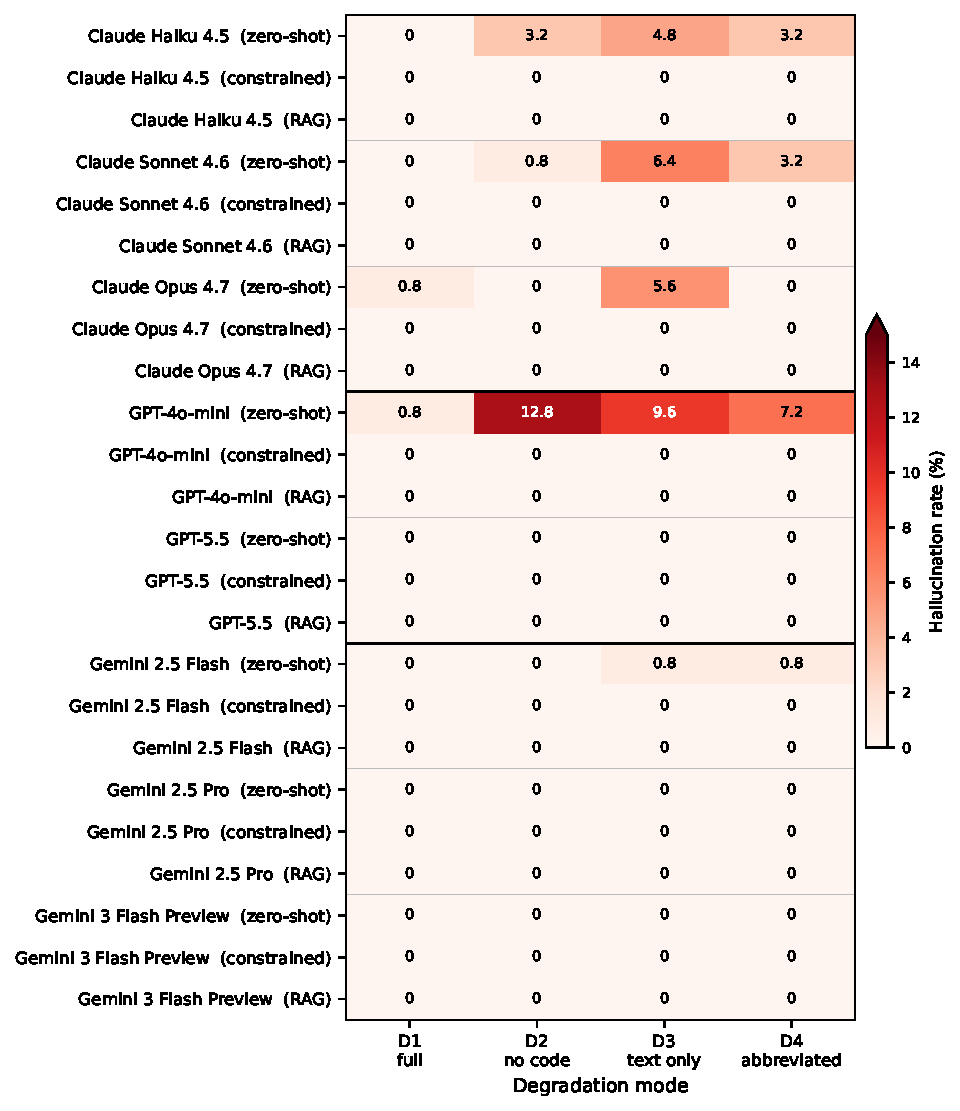
\includegraphics[width=0.85\textwidth,keepaspectratio]{figures/figure1_hallucination_heatmap.pdf}
\caption{Hallucination rate (\%) by model, prompting mode, and degradation mode. Each row is one (LLM, prompting mode) configuration; columns are the four degradation modes. Cell color encodes the percentage of D-mode predictions that were fabricated codes (predictions that do not exist in the FY2026 CMS-published ICD-10-CM tabular list). Constrained and RAG rows are uniformly zero across all Anthropic and OpenAI models. Zero-shot fabrication concentrates in sub-flagship models, peaking at 12.8\% for GPT-4o-mini under D2.}
\par\noindent\textit{Alt text: Heatmap with 24 rows (model and prompting mode) and 4 columns (degradation modes). Red color intensity encodes hallucination percentage; the numeric value appears in each cell.}
\label{fig:halluc}
\end{figure*}

Within-model paired comparison (zero-shot versus constrained,
McNemar tests on discordant pairs) confirms the constrained-mode
reduction is statistically significant for every Anthropic and
OpenAI model with nonzero zero-shot hallucination. Gemini 2.5 Pro
zero-shot exhibits a near-complete abstention pattern (95.2\%
no\_prediction at D4) with 0\% fabrication. The failure mode is
abstention, not fabrication, and constrained and RAG cut but do
not eliminate it. Whether this reflects model behavior or a
wrapper-level interaction with the reasoning-token budget is
unresolved (see §Discussion limitations). Gemini 2.5 Flash and
Gemini 3 Flash Preview zero-shot abstain rather than fabricate.
When these models do return a code under D2 to D4 stress, it is
almost always real (hallucination $\leq$0.8\% across all cells); the
dominant failure is empty-prediction, which rises to 39 to 42\%
under D4 abbreviation stress. Full 24-LLM tables in Supplementary
§S2.2 to §S2.3.

\subsection{Top-1 vs top-5 exact-match lift}\label{top-1-vs-top-5-exact-match-lift}

Many configurations have the right answer in their top-5
candidates even when their top-1 pick is wrong. Table 2 reports
top-1 accuracy, top-5 accuracy, and the resulting lift across
selected configurations.

\begin{table*}[!t]
\centering
\caption{Top-1 vs top-5 exact-match lift across selected configurations.}
\begin{tabular}{@{}llll@{}}
\toprule
Model & Top-1 & Top-5 & Lift \\
\midrule
claude-haiku-4-5 (constrained) & 96.8\% & 100.0\% & +3.2pp \\
claude-sonnet-4-6 (constrained) & 94.6\% & 100.0\% & +5.4pp \\
claude-opus-4-7 (constrained) & 94.8\% & 99.8\% & +5.0pp \\
gpt-4o-mini (constrained) & 94.2\% & 100.0\% & +5.8pp \\
gpt-5.5 (constrained) & 93.6\% & 100.0\% & +6.4pp \\
sentence-transformer:retrieval & 69.0\% & 90.6\% & +21.6pp \\
baseline:tfidf & 45.2\% & 83.2\% & +38.0pp \\
claude-sonnet-4-6 (zeroshot) & 75.4\% & 95.8\% & +20.4pp \\
gpt-5.5 (zeroshot) & 88.8\% & 98.8\% & +10.0pp \\
gemini-2.5-pro (zeroshot) & 11.8\% & 11.8\% & +0.0pp \\
\bottomrule
\end{tabular}
\end{table*}

Two patterns are visible. LLMs in \emph{constrained} mode saturate
at top-1 (lift $\leq$6pp), so there is little additional value in
human-in-the-loop top-5 review for those configurations.
Non-LLM baselines and sub-frontier LLMs in zero-shot mode show
much larger lifts (20 to 38pp), suggesting that workflows
surfacing top-5 candidates to a human reviewer would substantially
improve net accuracy. Gemini 2.5 Pro's zero lift is consistent
with the abstention-dominated failure mode, since there is no
candidate to be lifted into top-5 when the model returns nothing.

\subsection{Cost per correct prediction}\label{cost-per-correct-prediction}

Most prior LLM medical-coding benchmarks report accuracy in
isolation \autocite{Soroush2024,Almeida2025,Singh2025}. The deployment
decision, however, hinges on the joint distribution of API cost
per call, per-call accuracy, and the rate of failure modes that
drive downstream QA cost. Table 3 reports per-call API cost across
selected (model, prompting-mode) configurations from the headline
matrix; the full 28-configuration breakdown, per-bucket cost
decomposition, break-even analysis (LLM and QA versus a human
coder), and annual cost projections at deployment scale are
reported in Supplementary §S5.

\begin{table*}[!t]
\centering
\caption{Per-call API cost across selected (model, prompting-mode) configurations from the headline matrix. n = number of completed calls (out of 500 attempted). †, ‡ explained in the footnotes below.}
\begin{tabular}{@{}lrrr@{}}
\toprule
Model × Mode & n & \$ total & \$ per call (mean) \\
\midrule
claude-opus-4-7:zeroshot & 500 & 6.77 & 0.01354 \\
claude-sonnet-4-6:zeroshot & 500 & 3.41 & 0.00682 \\
claude-haiku-4-5:constrained & 500 & 2.14 & 0.00428 \\
gpt-5.5:zeroshot † & 499 & 3.59 & 0.00720 \\
gpt-4o-mini:constrained & 500 & 0.14 & 0.00028 \\
gemini-2.5-pro:zeroshot ‡ & 424 & 0.41 & 0.00096 \\
gemini-2.5-flash:zeroshot & 500 & 0.03 & 0.00005 \\
\bottomrule
\end{tabular}
\end{table*}

† One of 500 attempted gpt-5.5 zero-shot calls exhausted the SDK
retry budget on a transient API error and is excluded from the cost
total. We report n=499 as-is rather than re-running, since transient
API failures are an inherent property of production LLM deployment
and re-running would obscure that signal.

‡ Gemini 2.5 Pro zero-shot completed 424 of 500 attempted calls
under our wrapper's \texttt{max\_output\_tokens=1024} setting. The remaining
76 returned empty responses consistent with reasoning-token budget
exhaustion (counted as \texttt{no\_prediction} in §4.3, not as cost-bearing
calls). The 424 figure reflects calls that produced billable
output; cost normalization uses that denominator.

A 270× spread separates the cheapest configuration (Gemini 2.5
Flash zeroshot at \$0.00005/call) from the most expensive (Claude
Opus 4.7 zeroshot at \$0.01354/call). Per-call price varies more
dramatically across the matrix than per-call accuracy, so
cost-per-correct prediction is dominated by per-call price for any
configuration that achieves $\geq$80\% top-1 accuracy. One caveat: the
cost numbers reported here are \emph{automated-coding cost}, not the
broader role of clinical informaticists. Any break-even analysis
is \emph{deployment cost guidance}, not an \emph{automation feasibility
verdict}. Error tolerance is workflow-specific, and a hallucinated
code that flows into claims billing has different downstream cost
than the same hallucination in a research cohort definition. The
full caveats are in Supplementary §S5.

Cost-per-correct (\$ per exact-match outcome) collapses per-call
price and accuracy into one deployment-ready number; the Top-1
and Halluc columns surface all three deployment dimensions in one
row. Plotted as a Pareto frontier in Figure 2 and tabulated in
Table 4 below. Sorted by \$/correct ascending; n=500 per row.

\begin{figure*}[!t]
\centering
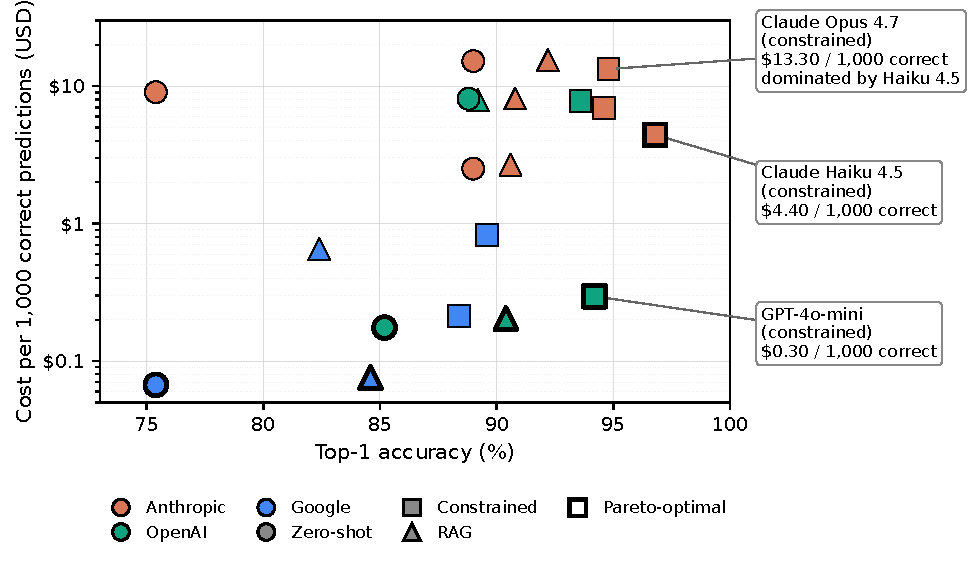
\includegraphics[width=0.9\textwidth,keepaspectratio]{figures/figure2_cost_frontier.pdf}
\caption{Cost per 1,000 correct predictions (USD, log scale) versus top-1 accuracy for every (LLM, prompting mode) configuration achieving \(\geq\)75\% top-1 accuracy. Color encodes provider; marker shape encodes prompting mode. Pareto-optimal configurations are drawn with a heavy black border. GPT-4o-mini constrained and Claude Haiku 4.5 constrained sit on the deployment frontier; Claude Opus 4.7 constrained is dominated despite competitive accuracy because its per-correct cost is 30 to 40 times higher.}
\par\noindent\textit{Alt text: Scatter plot of cost per 1,000 correct predictions on a logarithmic y-axis against top-1 accuracy on the x-axis. Provider is encoded by color, prompting mode by marker shape; Pareto-optimal configurations carry heavier black borders.}
\label{fig:cost}
\end{figure*}

\begin{table*}[!t]
\centering
\caption{Cost per correct prediction. \emph{constr.} = constrained. *Gemini 2.5 Pro constrained reflects abstention pattern, not error rate; see §4.3 (Failure-mode breakdown).}
\begin{tabular}{@{}
  >{\raggedright\arraybackslash}p{(\columnwidth - 10\tabcolsep) * \real{0.4267}}
  >{\raggedright\arraybackslash}p{(\columnwidth - 10\tabcolsep) * \real{0.1333}}
  >{\raggedleft\arraybackslash}p{(\columnwidth - 10\tabcolsep) * \real{0.0933}}
  >{\raggedleft\arraybackslash}p{(\columnwidth - 10\tabcolsep) * \real{0.1067}}
  >{\raggedleft\arraybackslash}p{(\columnwidth - 10\tabcolsep) * \real{0.0933}}
  >{\raggedleft\arraybackslash}p{(\columnwidth - 10\tabcolsep) * \real{0.1467}}@{}}
\toprule
\begin{minipage}[b]{\linewidth}\raggedright
Model
\end{minipage} & \begin{minipage}[b]{\linewidth}\raggedright
Mode
\end{minipage} & \begin{minipage}[b]{\linewidth}\raggedleft
Top-1
\end{minipage} & \begin{minipage}[b]{\linewidth}\raggedleft
Halluc
\end{minipage} & \begin{minipage}[b]{\linewidth}\raggedleft
Total
\end{minipage} & \begin{minipage}[b]{\linewidth}\raggedleft
\$/correct
\end{minipage} \\
\midrule
Gemini 2.5 Flash & rag & 84.6\% & 0.0\% & \$0.03 & \$0.0001 \\
GPT-4o-mini & zeroshot & 85.2\% & 7.6\% & \$0.07 & \$0.0002 \\
GPT-4o-mini & rag & 90.4\% & 0.0\% & \$0.09 & \$0.0002 \\
Gemini 2.5 Flash & constr. & 88.4\% & 0.0\% & \$0.09 & \$0.0002 \\
\textbf{GPT-4o-mini} & \textbf{constr.} & \textbf{94.2\%} & \textbf{0.0\%} & \textbf{\$0.14} & \textbf{\$0.0003} \\
Gemini 3 Flash Preview & constr. & 89.6\% & 0.0\% & \$0.37 & \$0.0008 \\
Claude Haiku 4.5 & rag & 90.6\% & 0.0\% & \$1.22 & \$0.0027 \\
Claude Haiku 4.5 & constr. & 96.8\% & 0.0\% & \$2.14 & \$0.0044 \\
Claude Sonnet 4.6 & constr. & 94.6\% & 0.0\% & \$3.26 & \$0.0069 \\
GPT-5.5 & constr. & 93.6\% & 0.0\% & \$3.63 & \$0.0078 \\
Gemini 2.5 Pro* & constr. & 46.2\% & 0.0\% & \$1.57 & \$0.0068 \\
Claude Opus 4.7 & constr. & 94.8\% & 0.0\% & \$6.31 & \$0.0133 \\
\bottomrule
\end{tabular}
\end{table*}

Reading the table top-down, the cheaper rows are all 4 to 19pp
lower on top-1 or carry nonzero hallucination. \textbf{GPT-4o-mini
constrained leads on deployment-relevance}: 94.2\% top-1, 0\%
hallucination, \$0.0003 per correct, the cheapest configuration
that achieves $\geq$94\% top-1. Claude Haiku 4.5 constrained adds 2.6pp
accuracy at roughly 14× the cost. Claude Opus 4.7 constrained's
0.6pp accuracy edge does not justify its 44× cost: the largest
frontier model is not the deployment leader. Gemini 2.5 Pro's
elevated \$/correct reflects abstention behavior, not a normal
cost-accuracy tradeoff.

\subsection{Outcome distribution under D4 abbreviation stress}\label{outcome-distribution-under-d4-abbreviation-stress}

D4\_abbreviated is the strongest stress test in the matrix.
Explicit ICD codes and canonical display strings are stripped,
and clinical entities are replaced with jargon (``T2DM'', ``HTN'',
``CKD-3''). String-matching baselines collapse (fuzzy and TF-IDF
both drop \textasciitilde30pp from D3 to D4), so remaining top-1 accuracy must
come from semantic mapping. Anthropic constrained mode holds up
under D4 (Haiku 93.6\%, Sonnet 90.4\%, Opus 86.4\% top-1, versus
100\% at D1), and the failure mode is exclusively \texttt{category\_match}.
Frontier zero-shot LLMs show a 5 to 15pp top-1 drop from D1 to D4
but maintain low hallucination. Gemini 2.5 Pro abstention worsens
monotonically from D1 to D4 across all three prompting modes.
Figure 3 shows the full six-bucket outcome distribution per
configuration under D4 stress.

\begin{figure*}[!t]
\centering
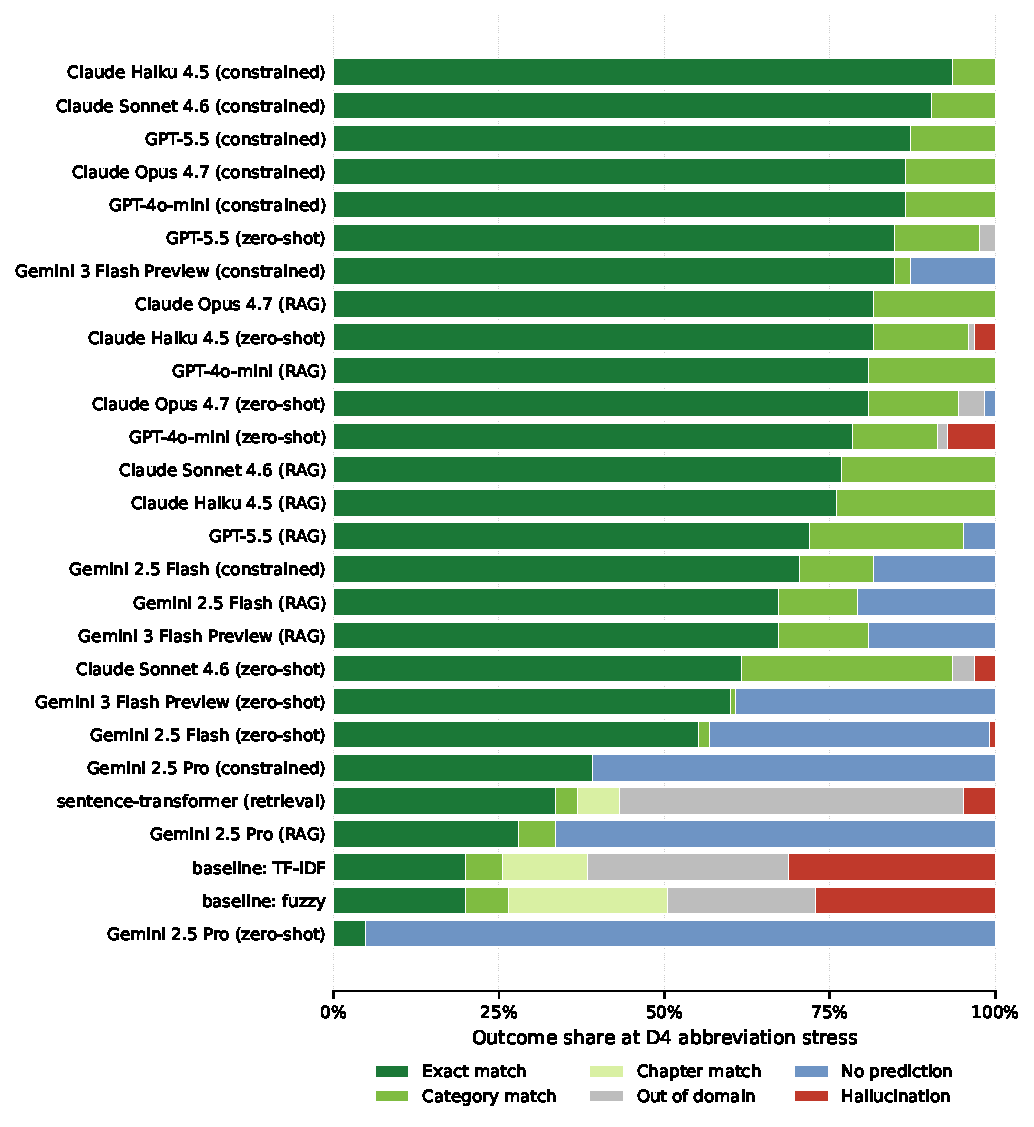
\includegraphics[width=0.75\textwidth,keepaspectratio]{figures/figure3_d4_outcome_stack.pdf}
\caption{Outcome distribution per (model, prompting mode) configuration under D4 abbreviation stress. Each horizontal bar sums to 100\% across the six outcome buckets defined in \S2.5; bars are ordered by exact\_match share descending. Anthropic and OpenAI constrained configurations cluster at the top, dominated by exact\_match with a small category\_match remainder. Gemini 2.5 Pro at the bottom is dominated by no\_prediction (abstention), distinct from the hallucination-heavy string-matching baselines (\texttt{baseline:fuzzy}, \texttt{baseline:tfidf}) below it.}
\par\noindent\textit{Alt text: Horizontal stacked bar chart with 27 rows (each model and prompting mode plus baselines), ordered top-down by descending exact-match share. Six color-coded segments per bar represent the outcome buckets defined in the methods section.}
\label{fig:d4stack}
\end{figure*}
\section{DISCUSSION}\label{discussion}

\subsection{Principal findings}\label{principal-findings}

The headline result is that \textbf{fabrication is bounded in modern
frontier LLMs and stratifies cleanly by model tier and prompting
mode}, while abstention is the more consequential failure mode
for some models. The 6-way taxonomy is what makes the second
pattern visible. Across the 24 LLM configurations, hallucination
ranges from 0\% to 5.6\% for flagship models (Opus 4.7, GPT-5.5,
Gemini 2.5 Pro) and from 0\% to 12.8\% for sub-flagship models, with
the upper bound from GPT-4o-mini zero-shot D2. Hallucination
behaves as a property of the prompting setup rather than a fixed
property of the model. The shift from zero-shot to constrained
prompting eliminates fabrication entirely for every Anthropic and
OpenAI model that shows any nonzero zero-shot hallucination, and
within-model paired McNemar tests confirm significance at n=125.
The string-matching baselines and the frozen sentence-transformer
baseline (45 to 69\% top-1) sit well below every constrained-mode
LLM on the fabrication-versus-accuracy frontier, confirming that
constrained frontier LLMs offer real gains over lexical and
embedding-only approaches at this cohort scale. Cost-per-correct
collapses the deployment choice to a small frontier: GPT-4o-mini
constrained at \$0.0003 and Claude Haiku 4.5 constrained at
\$0.0044 dominate every more expensive configuration tested.

\subsection{Comparison with prior work}\label{comparison-with-prior-work}

The closest direct precedent is Soroush et al.~(2024)
\autocite{Soroush2024}, who benchmarked four 2023--2024 vintage
LLMs on direct ICD code querying. Our matrix differs from theirs in
three ways relevant to deployment. The first is model generation.
Their headline numbers are GPT-4 (46\% exact match on ICD-9, 34\%
on ICD-10); our matrix includes Opus 4.7, GPT-5.5, and Gemini 3
Flash Preview on the same task type. Every Anthropic and OpenAI
configuration we evaluated exceeds 80\% top-1 even under the D4
abbreviation stress, which we attribute to cohort-scope
restriction, generational LLM improvements, and structured-output
prompting. The second is per-prediction cost. Soroush et al.\ and
the broader hallucination-mitigation literature
\autocite{DasBaksi2024,Sarvari2025,Motzfeldt2025,HybridCode2025} do
not report per-prediction cost; we do, and cost-per-correct
collapses the choice to a small Pareto frontier (GPT-4o-mini
constrained at \$0.0003 and Claude Haiku 4.5 constrained at
\$0.0044). The third is the outcome taxonomy: hallucination is an
explicit, mutually-exclusive bucket, abstention is split out via
the 6-way taxonomy, and the within-model zero-shot vs.\ constrained
vs.\ RAG contrast is reported as a controlled ablation that
separates ``wandering off the menu'' from genuine ignorance.
Neuro-symbolic alternatives \autocite{Motzfeldt2025,HybridCode2025}
report hallucination control through architectural constraints;
our 0\% Anthropic constrained-mode rate sits below their reported
neural-baseline band, suggesting that modern frontier LLMs under
structured-output constraints have closed much of the fabrication
gap those systems were designed to fix. Full comparison is in
Supplementary §S2.

\subsection{Implications for clinical deployment}\label{implications-for-clinical-deployment}

The 6-way taxonomy reframes the deployment question. Top-1
accuracy framing treats every wrong answer equally, but the cost
of a hallucinated code (downstream systems silently mishandle it,
propagating into billing, research, and quality reporting) is
qualitatively different from a near-miss within the correct ICD
chapter (corrected by a reviewer in seconds), which is in turn
different from an abstention (re-coding from scratch, but
emitting no spurious artifact).

The deployment pattern supported by these results is therefore
\textbf{LLM-augmented coding with terminologist or
clinical-informaticist review}, not autonomous LLM coding. Two
findings concretely support this. For constrained-mode Anthropic
and OpenAI configurations (0\% hallucination, \textasciitilde5\% category-match,
\textasciitilde0\% abstention), the QA fraction is dominated by fast
category-match adjudication, a clinically straightforward task an
experienced coder can resolve in seconds, which beats human-only
coding across all sensitivity-sweep parameter ranges considered
(Supplementary §S5). The top-1 vs top-5 lift table (§4.4) also
shows that trained-classifier and sub-frontier zero-shot LLM
workflows (top-1 in the 45 to 75\% range) benefit substantially
from surfacing top-5 candidates to a reviewer, lifting net
accuracy 20 to 38 percentage points. Constrained-mode frontier
LLMs already saturate top-1 (lift $\leq$6pp) and shift the reviewer's
role from candidate selection to category-match adjudication.
Either architecture keeps a clinical adjudicator in the decision
loop where accuracy matters most.

\subsection{Implications for semantic interoperability}\label{implications-for-semantic-interoperability}

Automated terminology grounding is a load-bearing component of
modern interoperability pipelines: HL7 FHIR, IHE profiles, and the
OMOP Common Data Model all presume that coded fields resolve to
entries in controlled vocabularies, and they degrade silently when
those resolutions fail. The 6-way outcome taxonomy has three
practical consequences for pipeline design. \emph{First}, the
\texttt{hallucination} bucket is a data-quality red flag for any
harmonization step: a fabricated code propagates into the
harmonized dataset undetected, silently corrupting cohort
definitions, billing aggregates, and downstream training data. The
\texttt{no\_prediction} bucket, by contrast, is a tractable gap
that surfaces as a missing value a reviewer or fallback heuristic
can resolve. Treating these as the same failure mode (as some prior
work does) under-counts the silent-corruption risk. \emph{Second},
cost-per-correct is a budget input for interoperability-pipeline
design. A pipeline processing 250,000 conditions/year at \$0.0003
per correct (GPT-4o-mini constrained) costs ~\$70/year in API
spend; the same pipeline at \$0.0133 per correct (Opus 4.7
constrained) costs ~\$3,300/year for the same accuracy floor. The
choice is not "which model is best" but "which (model, prompting
mode) point on the Pareto frontier matches the deployment
constraints." \emph{Third}, the 6-way taxonomy generalizes as a
reusable yardstick for any vocabulary-grounding component, not just
ICD-10-CM: LOINC for labs, RxNorm for medications, SNOMED CT for
broader clinical concepts. The bundled FY2026 CMS validator that
distinguishes hallucination from out-of-domain in our matrix has
direct analogs in the other vocabulary registries.

\subsection{Limitations}\label{limitations}

The v1 headline matrix evaluates n=125 unique Synthea Conditions.
Per-cell Wilson 95\% CIs on a 10\% rate are correspondingly ±5pp,
and v2 replication at n=2000 will tighten intervals by
approximately 2×. Gemini 2.5 Pro showed an 88\% no\_prediction
rate on zero-shot D4 with most empty rows showing zero output
tokens, consistent with reasoning-token budget exhaustion under
our wrapper's \texttt{max\_output\_tokens=1024} setting. Whether this is
a fixable wrapper interaction or a genuine model limitation is
the subject of a follow-up investigation blocked by Tier-1 daily
quota at v1 submission. Gemini 3.1 Pro Preview was excluded for
the same quota reason. The benchmark covers English ICD-10-CM
only; extension to LOINC and RxNorm via the same taxonomy is
planned for v2.

\subsection{Future directions}\label{future-directions}

Two extensions follow directly. The first is v2 vocabulary
expansion to LOINC and RxNorm; the 6-way taxonomy and eval runner
already support arbitrary FHIR resource types. The second is
rationale evaluation following Li et al.~\autocite{Li2025}, in
which each LLM is asked for a per-prediction rationale to support
faithfulness and plausibility evaluation alongside the
outcome-bucket framework. A v2 cohort with broader vocabulary and
more realistic clinical text (e.g., discharge summaries, ED notes)
is also needed to establish the true effect size of fabrication
risk on real clinical inputs.
\section{CONCLUSION}\label{conclusion}

Across a 24-LLM-configuration evaluation matrix on n=125
Synthea-generated FHIR Conditions, fabrication of non-existent
ICD-10-CM codes ranged from 0\% to 5.6\% for flagship models (Opus
4.7, GPT-5.5, Gemini 2.5 Pro) and from 0\% to 12.8\% for sub-flagship
models. Constrained prompting eliminated fabrication entirely for
every Anthropic and OpenAI model. Hallucination behaves as a
controllable property of the prompting setup at this scale rather
than a fixed model limitation. Abstention, separated from
fabrication via the 6-way taxonomy, proved the more consequential
failure mode for some models.

Two caveats temper the headline. The n=125 cohort and the narrow
12-code ACCESS-Model vocabulary limit per-cell precision and bound
the population that surfaces fabrication. The D4
abbreviation-substitution stress is only one proxy for real-world
hallucination triggers; multi-condition narratives, ambiguous
documentation, code-specificity ambiguity, and long-tail rare
diagnoses are not exercised here. A v2 cohort with broader
vocabulary and more realistic clinical text (e.g., discharge
summaries, ED notes) is needed to establish the true effect size
of fabrication risk on real clinical inputs.

Two recommendations follow from the matrix. \textbf{Zero-shot LLM prompting
is inferior to constrained and retrieval-augmented grounding for
medical concept normalization}, since every observed fabrication
occurred under zero-shot, and only the grounded configurations
eliminated it. Among
grounded configurations, \textbf{cost-per-correct rather than accuracy
alone should drive selection}, because clinical coding errors are
downstream-costly and the cheaper model can win on the combined
metric. The deployment frontier consists of \textbf{GPT-4o-mini
constrained} (94.2\% top-1, \$0.0003 per correct, the cheapest
configuration at $\geq$94\% accuracy) and \textbf{Claude Haiku 4.5
constrained} (96.8\%, \$0.0044 per correct, an additional 2.6pp
accuracy at roughly 14× the cost). Both dominate the largest
frontier model (Opus 4.7 constrained, 94.8\%, \$0.0133). The
supported workflow is LLM-augmented coding with terminologist
review.

% ─── Back-matter ───────────────────────────────────────────────────────

\section*{Acknowledgments}
\textbf{Use of AI tools.} This work used Anthropic's Claude (Claude
Code, model Claude Opus 4.7) as a coding, drafting, and
figure-design assistant during the development of the benchmark
codebase, the manuscript prose, and the figures. The author
conceived and designed the study, defined the experimental framework
and outcome taxonomy, conducted all analyses, and reviewed and
verified the AI-generated content. The author retains full
responsibility for the content, methodology, results, and any
errors.

\section*{Competing Interests}
The author declares no competing interests.

\section*{Funding}
This work received no external funding. LLM API access (Anthropic,
OpenAI, Google) for the evaluation matrix was self-funded by the
corresponding author; per-call costs are itemized in the Results
section.

\section*{Data Availability}
The Synthea-generated FHIR Bundles used for the headline evaluation
are freely redistributable and will be released as
\texttt{benchmarks/synthetic\_v1/} alongside the paper at
\url{https://github.com/ufbfung/phantom-codes}. All source code,
including the data-preparation pipeline, degradation logic,
ICD-10-CM validator, eval runner, prompts, and baselines, is
publicly available at the same repository under the MIT License.

\section*{Code Availability}
All source code, configuration files, synthetic test fixtures, and
the manuscript source are publicly available at
\url{https://github.com/ufbfung/phantom-codes} under the MIT
License. The repository includes the full evaluation pipeline and
the Synthea generation configuration needed to reproduce the
headline matrix end-to-end.

\printbibliography

\end{document}
